\section{Building our own tracking system using routers and hotspots}
This will cover the advancements that have been made in building and gather information using routers and hotspots, A list of objectives can be found in below. The goal for this is the enable us to calculate the positioning ourself and compare them to the current system Cisco.

An overview of the entire system can be see below in figure \ref{fig:OwnSetup} 
\begin{figure}[H]
	\centering
	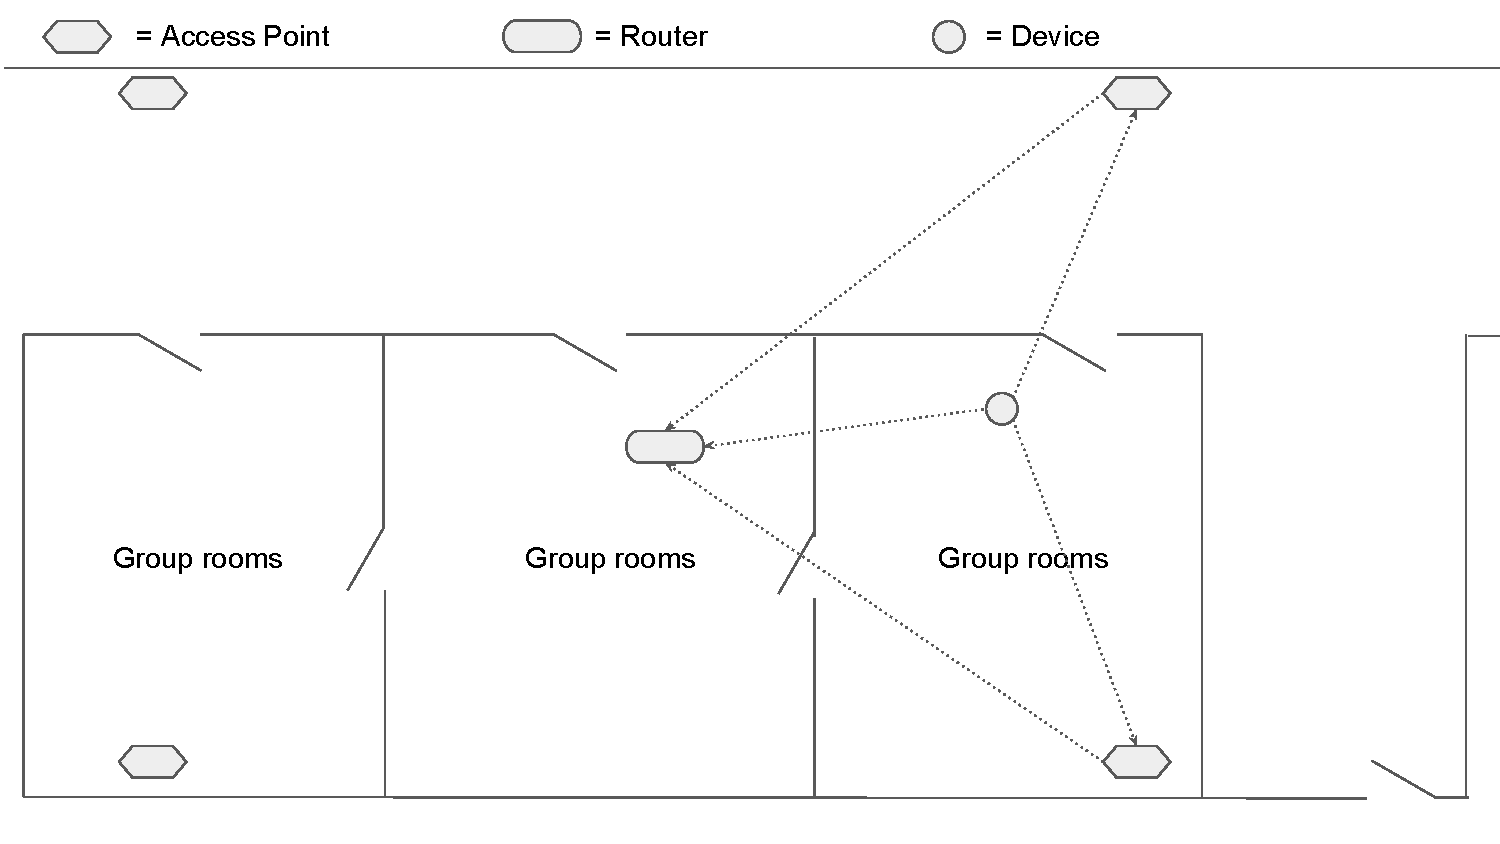
\includegraphics[scale=0.5]{graphics/Router-AccessPoint_Setup.pdf}
	\label{fig:OwnSetup}
	\caption{Illustration of how a positioning system can be setup using routers and access point that can track devices}
\end{figure}

\begin{itemize}
	\item Buying Equipment
	\item Test Capabilities of the Equipment
\end{itemize}

\subsection*{Buying Equipment}
The initial requirements for the equipment is that it needs to have a wireless antenna that should at least support 2.4 GHz and optionally 5 GHz, additionally we would need two be able to setup two different ILBS, we decided to buy two brands to also analyse which of the systems performed best based on the criteria describe in section \ref{sec:monitoring}.

Based on the above requirements we found two brands, D-link and Ubiquiti. We ordered one router, two expensive access points and five cheap access points of each brand. D-link is considered to be the cheaper brand then Ubiquiti.

\subsection*{Test Capabilities of the Equipment}
We tested the Ibiquiti equipment, with the original firmware. At first glance we are able to get transmission(TX) and receive(RX) signals of connected devices which is a good sign, unfortunately we do not receive the signals from the devices not connected to the router. We tried to use routers terminal which did not yield any results because of restricted access.

This lead to search about custom firmwares for the router that we ordered. By installing a new firmware on the router we will be able to get root access to the router and thereby manipulate the router at a lower level then the router original firmware allows, this is necessary if we not to capture every receive signal that the router gets.

We did find a custom firmware for Ibiquiti but not for D-link. The sites we have looked at were: openwrt.org, polarcloud.com, dd-wrt.com, gargolye-router.com, librecmc.org and wrtrouters.com These sites covers over thousands of routers and the fact we were not able to find a custom firmware for D-link might be because of that particular model we ordered because other routers from that brands were supported, nothing conclusion was found, to why it is not covered on any of the websites because.

We ended up going with the openwrt because it supported our Ibiquiti router and allow us to gain root access and execute programs. With the new custom firmware installed we have around 8mb of memory left this put some limitation to which language we can use, our first attempt is to use a version of python called mini-python that dose not exceed the memory limit.

A program is constructed that would allow us to listing on different types of networks like LAN and WAN, this is done using the socket library. But we were not able to import the library to our router which make the program on the router.